\section{A controlled, more demanding task}
\subsection{Sources, decisions and stress levels}
We generate original fictional company records with eight accounts each. The three query scenarios activate four, six and eight accounts, increase corporate distractors and source conflicts, and allow respectively 16, 12 and 8~KiB of UTF-8 evidence. These are compound stress levels; their differences cannot identify the causal effect of one difficulty factor. They are counterfactual task snapshots, not longitudinal observations. Three sector labels are administrative sampling strata under the same formal schema.

Each action requires an allowed region and sector, approved policy, observed consent and signal, and a complete account $\rightarrow$ initiative $\rightarrow$ need $\rightarrow$ offering $\rightarrow$ proof chain. Proof must be approved. Some actions additionally require operational capacity, permission to share proof, or assurance evidence. Thus useful evidence can come from operations, legal or engineering, as well as marketing. Current conflicts block the affected requirement. Unapproved policy suggestions, non-response observations, future corrections and restricted notes must not become current authorized facts.

The shared catalog contains six actions with known resource costs and policy multipliers. A plan selects at most three actions for distinct accounts within one shared budget. Its value is the sum of each account's approved priority multiplied by the selected action's multiplier. These are \emph{constructed policy points}, with no calibrated relationship to commercial outcomes. Multiple plans can attain the same optimum. Readers must cite every required source, including each link and the approved priority.

The dataset is machine-authored. It has no independent human annotation or independently authored test narratives. A fresh main seed creates new worlds after development, but the relation schema, catalog and generator remain known. More worlds improve precision within this generator; they do not establish generalization to real companies or unseen task families. We separately retain the earlier exploratory raw-document/wiki evaluation on externally authored fictional company material.

\subsection{Memory treatments and shared boundaries}
All retrieval methods receive identical visible records. A common current-view layer enforces valid time, observed time, permissions and explicit same-authority supersession. Records carry entity, relation, value, authority and source identifiers. This controlled ingestion boundary removes extraction errors from the main comparison.

\begin{table}[t]
\small\centering
\begin{tabularx}{\linewidth}{lX}
\toprule
Treatment & Actual implementation and comparison boundary \\
\midrule
No company context & Shared task/catalog with no company evidence; information reference. \\
Company context & Pinned native GBrain hybrid ranking followed by domain-neutral entity/link closure, up to four link steps. \\
GTM context & The same ranking, account order and packer, with closure restricted to relations required by the shared catalog. \\
Company + query words & Generic relation filtering using words in the shared query/glossary; no GTM allowlist. Exact input equivalence is audited before aliasing any reader output. \\
Markdown control & Lossless entity-wiki representation, BM25/dense rank fusion and the same generic entity closure. \\
GBrain search & Native hybrid ranking and bounded packing alone. \\
Full current context & All permitted current records; an explicitly larger information/cost reference. \\
\bottomrule
\end{tabularx}
\caption{Controls remain visible. GBrain denotes its pinned search component with shared verified records and real embeddings, not the complete agent, graph-ingestion pipeline or hosted product. The Markdown control is an original compatible record pattern, not an official Karpathy implementation.}
\label{tab:methods}
\end{table}

The GBrain component uses PGLite and balanced hybrid search at revision \texttt{531b3b1}; query expansion and reranking are disabled. Every retrieval system uses the same real \texttt{text-embedding-3-small} vectors with 1,024 dimensions. The typed selector follows relation names and entity links, never consent truth values, priorities, eligibility labels or optimal plans. The generic query-word control receives the same task glossary. Conflicting records for a selected slot travel together. Partial slot removal cannot make a conflict disappear. A deterministic byte packer makes the input allowance auditable; actual provider tokens are also measured.

\begin{figure}[t]
\centering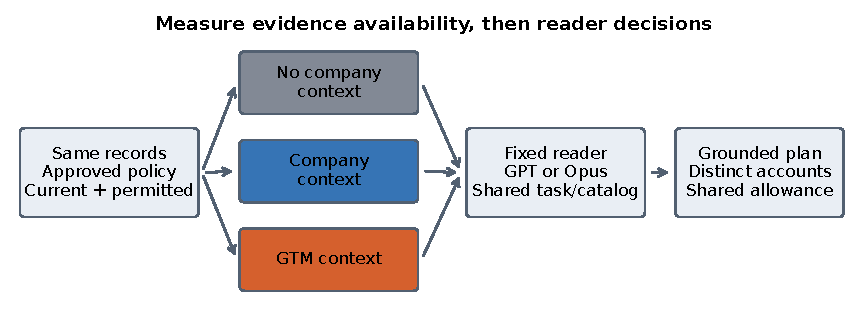
\includegraphics[width=\linewidth]{figures/challenge/design.pdf}
\caption{A common source bank and reader isolate context selection. We first compute what the selected evidence can support, then evaluate the returned plan against the full current facts and its supplied citations. The reference optimizer is a diagnostic over clean facts, not an agent baseline.}
\label{fig:design}
\end{figure}

\subsection{Readers, outcomes and uncertainty}
The new readers are \texttt{gpt-6.1-sol} with medium reasoning and \texttt{claude-opus-5-5} with adaptive thinking and high effort. Both exact model IDs and structured-output settings passed actual API checks. Each response allows up to 8,192 generated tokens; settings and prompts are constant across context treatments within a reader. Provider effort settings are not claimed compute-equivalent. There is one response per case/treatment/reader, with no automatic retries, answer repair or selection of a best attempt.

Let $V^*(q)$ be the maximum feasible policy value under full current information, $V^*_C(q)$ the maximum supported by selected context $C$, and $V_R(q)$ the value of the reader's fully grounded feasible plan. Our primary outcome is $V_R/V^*$ on cases with $V^*>0$; $V^*_C/V^*$ diagnoses evidence recoverability. An ineligible action, missing required citation, duplicate account or global budget violation invalidates the plan. Extra supplied citations are allowed, so the metric tests required-source completeness rather than citation minimality. Zero-optimum cases have a separate safety denominator. We also report exact optima, actionable coverage, abstention, failures, timing and costs. This is source-binding validation over formal records, not free-text entailment judgment or human-rated usefulness.

A development pilot covers 12 worlds and all treatments. The prospective sample rule uses the larger pilot company-level paired standard deviation across readers, targets an approximate five-percentage-point 95\% half-width, rounds to a multiple of three, and bounds the main size to 120--192 worlds. The main dataset, methods, settings and analysis are frozen before generation. The final main sample is \ChallengeWorlds{} worlds, \ChallengeCases{} cases and \ChallengeCalls{} actual reader attempts. We average positive cases within company, then weight companies equally. Confidence intervals resample companies within administrative strata, with 10,000 bootstrap replicates. The two GTM-minus-Company reader contrasts use paired random-sign tests with Holm adjustment; other contrasts are descriptive. Shared-template uncertainty is not real-market uncertainty.

An independently implemented SQLite query checks visibility and eligibility; exhaustive enumeration checks the dynamic-programming optimum. These are independent implementation checks by the same research assistant, not independent human validation. All raw responses and unsuccessful attempts remain in the artifact. Saved-output reproduction does not require paid model access; fresh inference is documented separately.
